\documentclass[10pt,a4paper]{article}

% ==========================================
% PACKAGES
% ==========================================
\usepackage[utf8]{inputenc}
\usepackage[T1]{fontenc}
\usepackage[english]{babel}
\usepackage[margin=2.2cm]{geometry}
\usepackage{graphicx}
\usepackage{amsmath,amssymb}
\usepackage{array}
\usepackage{longtable}
\usepackage{xcolor}
\usepackage{placeins}
\usepackage{needspace}
\usepackage{fancyhdr}
\usepackage{tikz}
\usetikzlibrary{positioning}

% ==========================================
% COLORS
% ==========================================
\definecolor{datasheetblue}{rgb}{0.07,0.21,0.35}
\definecolor{lightblue}{rgb}{0.90,0.94,0.98}

% ==========================================
% DOCUMENT CONFIGURATION
% ==========================================
\setlength{\parindent}{0pt}
\setlength{\parskip}{6pt}
\setlength{\tabcolsep}{6pt}
\renewcommand{\arraystretch}{1.25}

\pagestyle{fancy}
\fancyhf{}
\fancyhead[L]{\small ANALOG ONE}
\fancyhead[R]{\small Class AB Audio Amplifier}
\fancyfoot[L]{\small Technical Datasheet}
\fancyfoot[R]{\small Page \thepage}
\renewcommand{\headrulewidth}{0.4pt}

\setlength{\headheight}{14pt}

% Section formatting without titlesec
\newcommand{\datasheetsection}[1]{%
    \FloatBarrier%
    \par\addvspace{0.30cm}%
    \Needspace{5\baselineskip}%
    \noindent{\large\bfseries\color{datasheetblue}#1}\par%
    \vspace{0.10cm}%
    \hrule%
    \vspace{0.15cm}%
}

\newcommand{\datasheetsubsection}[1]{%
    \par\addvspace{0.15cm}%
    \Needspace{3\baselineskip}%
    \noindent{\normalsize\bfseries\color{datasheetblue}#1}\par%
}

\raggedbottom

\begin{document}

% ==========================================
% TITLE
% ==========================================
\begin{center}

{\Large\bfseries\color{datasheetblue}
AnalogOne}

\vspace{0.3cm}

{\Huge\bfseries Technical Datasheet}

\vspace{0.2cm}

{\Huge\bfseries 20W CLASS AB AUDIO AMPLIFIER}

\vspace{0.2cm}

{\large
Discrete-Component Audio Amplifier}

\vspace{0.2cm}

{\large
8 $\Omega$ Loudspeaker Application}

\vspace{0.4cm}

\end{center}

% ==========================================
% GENERAL DESCRIPTION
% ==========================================
\datasheetsection{General Description}

The AnalogOne Class AB Audio Amplifier is a 20W mono audio amplifier
designed to increase audio signal amplitude of a standard music player device with a 3.5mm Jack connector audio to power an 8 $\Omega$ nominal impedance Loudspeaker. The main quality feature is the capacity to maintain the audio signal with a THD of $0.88\%$ consider a good/moderate distortion useful for this application. The Amplifier runs off nominal symmetrical $\pm24$ V power supplies that ensure the power delivery to the speaker. The amplifier consists of three functional stages: a BJT preamplifier, a MOSFET voltage amplification stage, and a complementary MOSFET Class AB power output stage.

% ==========================================
% FEATURES
% ==========================================
\datasheetsection{Key Features}
\begin{itemize}
\item 20W with $0.88\%$ THD Output into a 8 $\Omega$ Load at $1kHz$.
\item 8 $\Omega$ nominal loudspeaker load.
\item Adjustable Volume Control.
\item Adjustable MOSFET bias.
\end{itemize}

% ==========================================
% Aplications
% ==========================================
\datasheetsection{Applications}
\begin{itemize}
\item Multi-Media Speaker System.
\item Music Amplifier.
\item Analog Audio Module.
\item Analog Sound Drive.
\end{itemize}

% ==========================================
% FUNCTIONAL DIAGRAM
% ==========================================
\datasheetsection{Functional Block Diagram}
\begin{figure}[htbp]
\centering

\resizebox{0.95\textwidth}{!}{%

\begin{tikzpicture}[
    node distance=0.8cm,
    block/.style={
        draw=datasheetblue,
        fill=none,
        thick,
        rectangle,
        rounded corners=2pt,
        align=center,
        minimum height=1.5cm,
        minimum width=3.0cm,
        inner sep=5pt
    },
    inputblock/.style={
        align=center,
        minimum height=1.5cm,
        minimum width=2.0cm
    },
    arrow/.style={
        ->,
        thick,
        >=latex
    }
]

% Audio input
\node[inputblock] (input) {
    \textbf{AUDIO INPUT}
};

% Preamplifier
\node[block, right=of input] (preamp) {
    \textbf{BJT PREAMPLIFIER}\\
    2N2222 Common-Emitter Stage
};

% Voltage amplifier
\node[block, right=of preamp] (vamp) {
    \textbf{VOLTAGE AMPLIFIER}\\
    IRF530 / IRF9540
};

% Class AB power stage
\node[block, right=of vamp] (power) {
    \textbf{CLASS AB POWER STAGE}\\
    IRFZ44N / IRF4905
};

% Loudspeaker
\node[block, right=of power] (speaker) {
    \textbf{8 $\Omega$ LOUDSPEAKER}
};

% Connections
\draw[arrow] (input.east) -- (preamp.west);
\draw[arrow] (preamp.east) -- (vamp.west);
\draw[arrow] (vamp.east) -- (power.west);
\draw[arrow] (power.east) -- (speaker.west);

\end{tikzpicture}%
}

\caption{Functional Block Diagram of the Device}
\label{fig:functional_block_diagram}

\end{figure}

\newpage
% =========================================================
% Device Circuit Architecture
% ========================================================
\datasheetsection{Device Circuit Architecture}
\begin{figure}[htbp]
\centering
\resizebox{0.95\textwidth}{!}{%
\begin{tikzpicture}
\node[
    anchor=south west,
    inner sep=0
] (circuit) at (0,0)
{
    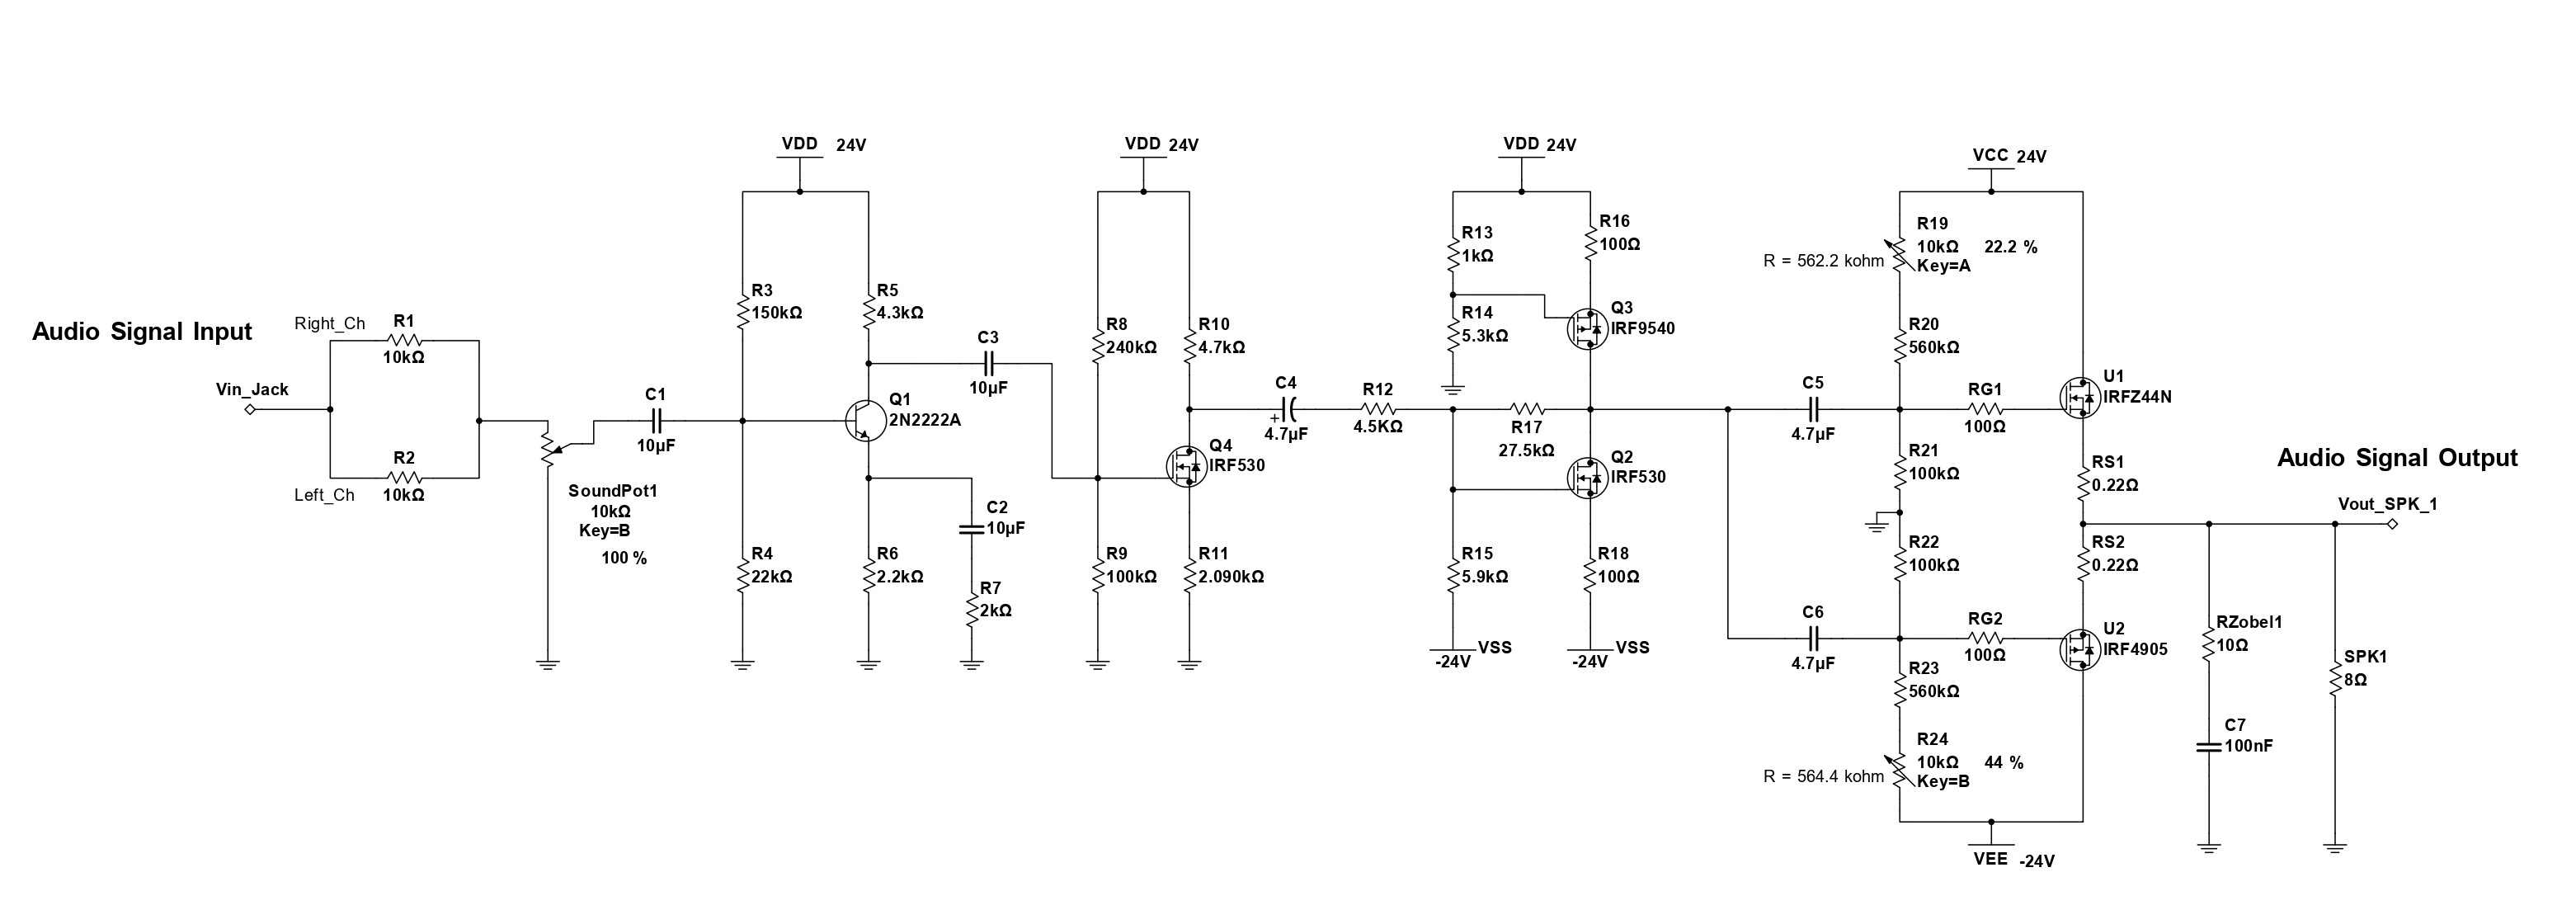
\includegraphics[width=\textwidth]{fig/Esquematico.jpg}
};

\begin{scope}[
    x={(circuit.south east)},
    y={(circuit.north west)}
]

% Separador Preamplificador
\draw[
    dashed,
    thin,
    datasheetblue
]
(0.195,0.05) -- (0.195,0.89);

% Separador Amplificador de voltaje
\draw[
    dashed,
    thin,
    datasheetblue
]
(0.40,0.05) -- (0.40,0.89);

% Separador Etapa de potencia
\draw[
    dashed,
    thin,
    datasheetblue
]
(0.66,0.05) -- (0.66,0.89);

% Títulos
\node[
    fill=white,
    text=datasheetblue,
    font=\bfseries\small
]
at (0.30,0.94)
{PREAMPLIFIER};

\node[
    fill=white,
    text=datasheetblue,
    font=\bfseries\small
]
at (0.53,0.94)
{VOLTAGE AMPLIFIER};

\node[
    fill=white,
    text=datasheetblue,
    font=\bfseries\small
]
at (0.82,0.94)
{CLASS AB POWER STAGE};

\end{scope}

\end{tikzpicture}
}
\caption{Device Circuit Architecture Modular Division}
\label{fig:amplifier_functional_division}

\end{figure}

% ==========================================
% COMPONENT SUMMARY
% ==========================================

\datasheetsection{Component Summary}
\small
\begin{longtable}{p{5.0cm}p{2.8cm}p{5.5cm}}
\hline
\textbf{Component Type} &\textbf{Component} &\textbf{Function} \\
\hline

\multicolumn{3}{l}{\textbf{Preamplifier Stage}} \\
\hline

NPN Transistor & 2N2222 & Common-emitter voltage amplification \\
\hline

\multicolumn{3}{l}{\textbf{Voltage Amplification Stage}} \\
\hline
N-Channel MOSFET &IRF530 &Voltage amplification \\
P-Channel MOSFET &IRF9540 &Active load for the voltage amplification stage \\
\hline

\multicolumn{3}{l}{\textbf{Class AB Power Stage}} \\
\hline
N-Channel MOSFET &IRFZ44N &Positive output current delivery \\
P-Channel MOSFET &IRF4905 &Negative output current delivery \\
Source Resistor &0.22 $\Omega$, 5 W & Current stabilization and source degeneration \\
Gate Resistor &100 $\Omega$ &Limits gate current and improves MOSFET stability \\
Bias Trimmer &10 k$\Omega$ &Adjustment of the Class AB quiescent bias \\
Coupling Capacitor &4.7 $\mu$F &Blocks DC while allowing the audio signal to pass \\
\hline

\multicolumn{3}{l}{\textbf{Output Network}} \\
\hline
Zobel Resistor &10 $\Omega$, 2 W &Output stabilization at high frequencies \\
Zobel Capacitor &100 nF &Forms the Zobel stabilization network with the 10 $\Omega$ resistor \\
\hline

\multicolumn{3}{l}{\textbf{Load}} \\
\hline
Loudspeaker &8 $\Omega$, 30 W &Nominal audio output load \\
\hline
\caption{Main amplifier components organized by functional stage of the device}
\label{tab:component_summary}
\end{longtable}
\normalsize
\newpage
% =========================================================
% GENERAL SYSTEM ELECTRICAL SPECIFICATIONS
% =========================================================
\datasheetsection{Electrical Specifications}

\begin{table}[htbp]
\centering
\small
\begin{tabular}{p{8.0cm}p{3.0cm}cc}
\hline
\multicolumn{3}{c}{\textbf{General Electrical Specifications of the Device}} \\
\hline
\textbf{Parameter} & \textbf{Value} & \textbf{Unit} \\
\hline
Supply voltage & $\pm24$ & V \\
Current Requiered & $-$ & A \\
Power Consumption & $-$ & W \\
RMS input voltage &  $1$--$2$ & V$_{\mathrm{RMS}}$ \\
Max RMS output voltage & 12.65 & V$_{\mathrm{RMS}}$ \\
Max RMS output current & 1.58 & A$_{\mathrm{RMS}}$ \\
Frecuency Range & $40$--$20k$ & Hz \\
Total harmonic distortion (THD) at 1 kHz & $0.88$ & \% \\
Reference output power     & 20 & W \\
Power efficiency & $-$ & \% \\
Nominal load resistance    & 8 & $\Omega$ \\
\hline
\end{tabular}
\label{tab:general_electrical_specs}
\end{table}

% =========================================================
% POWER DISIPATION & THERMAL - SPECIFICATIONS
% =========================================================
\datasheetsection{Power and Thermal Characteristics}

\begin{table}[htbp]
\centering
\small
\begin{tabular}{p{5cm}p{2cm}p{3cm}p{1.8cm}}
\hline
\textbf{Component} &\textbf{Device} &\textbf{Power Dissipation} &\textbf{$R_{\theta JC}$} \\
\hline

\multicolumn{4}{l}{\textbf{Preamplifier Stage}} \\
\hline
BJT Transistor & 2N2222 & 9.42 mW & -- \\
\hline

\multicolumn{4}{l}{\textbf{Voltage Amplification Stage}} \\
\hline
N-Channel MOSFET &IRF530 &-- &-- \\
N-Channel MOSFET &IRF530 &-- &-- \\
P-Channel MOSFET &IRF9540 &-- &-- \\
\hline

\multicolumn{4}{l}{\textbf{Class AB Power Stage}} \\
\hline
N-Channel MOSFET &IRFZ44N &6.58 W &1.5 $^\circ$C/W \\
P-Channel MOSFET &IRF4905 &6.63 W &0.75 $^\circ$C/W \\
\hline

\textbf{Output Stage Total} &-- &\textbf{13.21 W} &-- \\
\hline
\end{tabular}

\caption{Power dissipation and thermal characteristics of the amplifier stages.}
\label{tab:power_thermal_characteristics}

\end{table}

% ==========================================
% PERFORMANCE VERIFICATION
% ==========================================
\datasheetsection{13. Performance Verification}

The documented electrical results
were obtained through circuit simulation.

The Class AB power-stage reference
simulation used a 10 kHz input signal
and an 8 $\Omega$ load.

The recorded average output power
was 22.8 W.

The voltage amplification stage
was separately evaluated using
a 2 V RMS input signal at 1 kHz.

The simulated voltage gain was
7.118 V/V, with total harmonic
distortion of 1.183\%.

These results correspond to
individual stage evaluations.

Further testing is necessary
to determine the complete
amplifier frequency response,
harmonic distortion, noise,
and continuous output-power rating.

% ==========================================
% DOCUMENT INFORMATION
% ==========================================
\datasheetsection{14. Document Information}

\begin{tabular}{ll}
\hline
Developer & Analog One\\

Product & Class AB Audio Amplifier\\

Institution & Tecnologico de Costa Rica\\

Department & School of Electronics Engineering\\

Document & Technical Datasheet\\

Status & Design and Simulation\\
\hline
\end{tabular}

\vspace{0.8cm}

\begin{center}

\textcolor{datasheetblue}{
\textbf{
ANALOG ONE -- AUDIO AMPLIFICATION SYSTEM
}
}

\end{center}
\FloatBarrier
\end{document}
